
%dash pattern=on 5pt off 2pt
%[fill = white, rounded corners = 4pt, inner sep = 1pt]
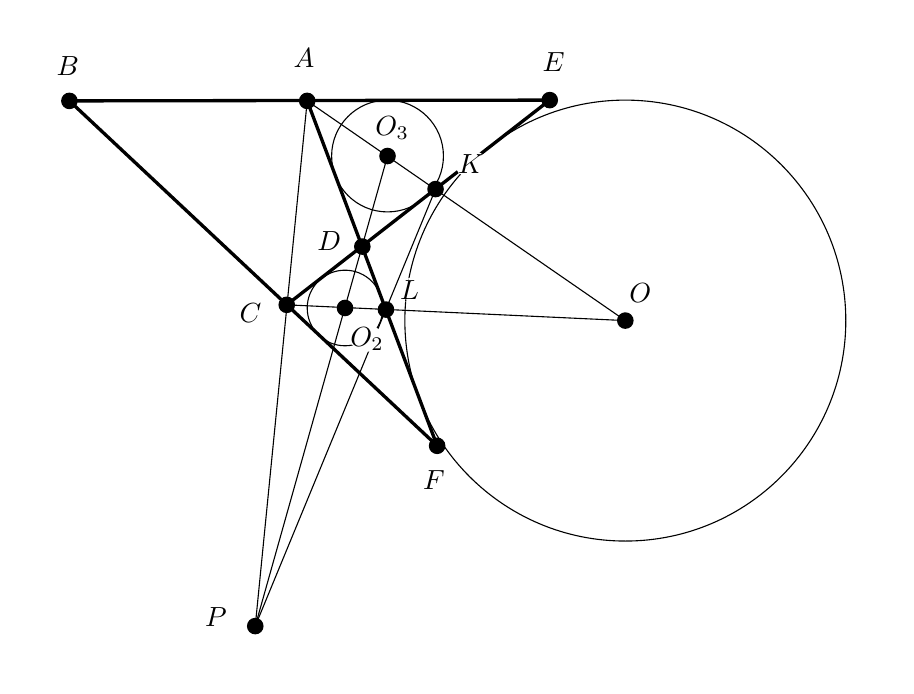
\begin{tikzpicture}[scale = 1]
    \clip(13.07,-0.17) rectangle (23.97,7.93);
    \draw(20.66,4.21) circle (2.8cm);
    \draw(17.1,4.37) circle (0.48cm);
    \draw(17.64,6.3) circle (0.71cm);
    \draw (16.62,7)-- (15.96,0.33);
    \draw (15.96,0.33)-- (17.64,6.3);
    \draw[line width=1.2pt] (18.27,2.62)-- (16.62,7);
    \draw[line width=1.2pt] (19.7,7.01)-- (16.36,4.41);
    \draw (20.66,4.21)-- (16.36,4.41);
    \draw (16.62,7)-- (20.66,4.21);
    \draw (15.96,0.33)-- (18.25,5.88);
    \draw[line width=1.2pt] (13.6,7)-- (19.7,7.01);
    \draw[line width=1.2pt] (13.6,7)-- (18.27,2.62);
    \begin{scriptsize}
        \normalsize
        \fill [color=black] (20.66,4.21) circle (3.0pt);
        \draw[color=black] (20.85,4.56) node {$O$};
        \fill [color=black] (13.6,7) circle (3.0pt);
        \draw[color=black] (13.58,7.44) node {$B$};
        \fill [color=black] (16.62,7) circle (3.0pt);
        \draw[color=black] (16.58,7.54) node {$A$};
        \fill [color=black] (18.27,2.62) circle (3.0pt);
        \draw[color=black] (18.23,2.19) node {$F$};
        \fill [color=black] (19.7,7.01) circle (3.0pt);
        \draw[color=black] (19.75,7.49) node {$E$};
        \fill [color=black] (16.36,4.41) circle (3.0pt);
        \draw[color=black] (15.9,4.3) node {$C$};
        \fill [color=black] (17.32,5.15) circle (3.0pt);
        \draw[color=black] (16.9,5.22) node {$D$};
        \fill [color=black] (17.62,4.35) circle (3.0pt);
        \draw[color=black] (17.92, 4.6) node[fill = white, rounded corners = 6pt, inner sep = 0.8pt] {$L$};
        \fill [color=black] (18.25,5.88) circle (3.0pt);
        \draw[color=black] (18.7,6.2) node[fill = white, rounded corners = 4pt, inner sep = 1pt] {$K$};
        \fill [color=black] (15.96,0.33) circle (3.0pt);
        \draw[color=black] (15.46,0.45) node {$P$};
        \fill [color=black] (17.1,4.37) circle (3pt);
        \draw[color=black] (17.38, 3.98) node[fill = white, rounded corners = 6pt, inner sep = 0.5pt] {$O_2$};
        \fill [color=black] (17.64,6.3) circle (3.0pt);
        \draw[color=black] (17.7,6.65) node[fill = white, rounded corners = 6pt, inner sep = 0.5pt] {$O_3$};
    \end{scriptsize}
\end{tikzpicture}